\documentclass[12pt]{article}
\usepackage{url,amsmath}
\usepackage{algorithm}
\usepackage{algpseudocode}
\usepackage{array}
\usepackage{amssymb}
\usepackage{amsbsy}
\usepackage{longtable}
\usepackage{graphicx}

\renewcommand{\algorithmicrequire}{\textbf{Input:}}
\renewcommand{\algorithmicensure}{\textbf{Output:}}

\setlength{\oddsidemargin}{.25in}
\setlength{\evensidemargin}{.25in}
\setlength{\textwidth}{6.25in}
\setlength{\topmargin}{-0.4in}
\setlength{\textheight}{8.5in}

\newcommand{\heading}[5]{
   \renewcommand{\thepage}{#1-\arabic{page}}
   \noindent
   \begin{center}
   \framebox{
      \vbox{
    \hbox to 5.78in { {\bf Math/Stat 310: Intro to Mathematical Statistics}
         \hfill #2 }
       \vspace{4mm}
       \hbox to 5.78in { {\Large \hfill #5  \hfill} }
       \vspace{2mm}
       \hbox to 5.78in { {\it #3 \hfill #4} }
      }
   }
   \end{center}
%   \vspace*{4mm}
}

\newcommand{\handout}[3]{\heading{#1}{#2}{Instructor:
Hyunseung Kang}{Scribe: Meenmo Kang}{Lectures #1: #3}}

\setlength{\parindent}{0in}
\setlength{\parskip}{0.1in}

\newcommand{\Var}{{\rm Var}}
\newcommand{\E}{{\rm E}}
\newcommand{\Cov}{{\rm Cov}}
\newcommand{\Corr}{{\rm Corr}}
\newcommand{\pdf}{{\rm pdf}}
\newcommand{\mgf}{{\rm MGF}}
\newcommand{\proof}{{\bf Proof. }} %% To begin a proof write \proof
\newcommand{\qed}{\mbox{}\hspace*{\fill}\nolinebreak\mbox{$\rule{0.6em}{0.6em}$}} %%to end your proof write $\qed$.
\newcommand{\ma}{{\mathcal A}}
\newcommand{\mf}{{\mathcal F}}
\newcommand{\hs}{\heartsuit}
\newcommand{\cs}{\clubsuit}
\newcommand{\noi}{\noindent}
\newtheorem{lemma}{Lemma}
\newtheorem{theorem}[lemma]{Theorem}
\newtheorem{definition}{Definition}
\newtheorem{proposition}{Proposition}
\newtheorem{remark}{Remark}

\bibliographystyle{plain}

\makeatletter
\newcommand*{\rom}[1]{\expandafter\@slowromancap\romannumeral #1@}
\makeatother
\begin{document}
\handout{12\&13}{March 12/14, 2018}{MLE \& Hypothesis Testing}
%Set n to the lecture number

\begin{section}{Properties of MLE}
In line with the last week, let's discuss about a couple more properties of MLE.
\subsection{Invariance of MLE}
\textbf{Theorem}\\
Given any function g: $\mathbb{R}\rightarrow\mathbb{R}$, if $\hat{\theta}_{MLE}$ is the MLE of $\theta$ from $pdf_{\theta}$ then $g(\hat{\theta}_{MLE})$ is the MLE of $g(\theta)$. 

\textbf{Example} \\
Let us get back to our favorite example again, measuring students' height on campus. Suppose that samples are normally and $i.i.d.$ distributed like $X_1,...,X_n \stackrel{iid}{\sim} N(\mu,\sigma^2)$. 
As we discovered last week, $\hat{\theta}_{MLE} = \frac{1}{n}\sum_{i=1}^n X_i = \bar{X}$ is for estimation of $\mu$. Now, we want to estimate $sin(\mu)$.\\

In a naive way, we could probably rewrite the density function $\frac{1}{\sqrt{2\pi\sigma^2}}exp \left(-\frac{(X_i-\mu)^2}{2\sigma^2}\right)$ in terms of $sin(\mu)$ in order to optimize the value. However, simply plugging $sin(\mu)$ into the normal density function is unable since $sin(\mu)$ is an invertible function. Instead, as long as we figure out a MLE, a MLE of $sin(\mu)$ is simply $sin(\hat{\mu}_{MLE})$.

\textbf{Example}\\
Suppose $X_i$ is income of $i$th individual, and we collect $n$ $i.i.d.$ samples. One of popular economics topics is distribution of income. Typically, the income distribution is not normal. So, in order for income distribution to be more like normal, log transformation is used as a method. As a result, normally and $i.i.d.$ log transformed samples are expressed as below. $$log(X_1),...,log(X_n) \stackrel{iid}{\sim} N(\mu,\sigma^2)$$

However, what we want to estimate is population mean income in \$ scale, not log\$ scale. At this point, we can come up with the fact that exponential to the log(A) is just A. Hence, in order for MLE estimator of $\mu$ in log scale, $\hat{\mu}_{MLE} = \frac{1}{n}\sum_{i=1}^n \log X_i $ to be transformed in an original scale, we can take exponential, such as $$\hat{\mu}_{MLE} (original\;scale) = exp(\frac{1}{n}\sum_{i=1}^n \log X_i)$$. $$\mu_{orignal\;scale} = exp(\mu_{log\;sclae})$$


%$$\includegraphics[height=4cm, width=12cm]{{Lec12&13_MLE&HypothesisTesting/a.png}}$$
\begin{figure}
    \centering
    \includegraphics[height=4cm, width=12cm]{a.png}
\end{figure}
\section{Point Estimate Optimality}
Let's review the two different methods of estimating parameter that we have covered.
\begin{itemize}
	\item MOM Estimator: $\hat{\theta}_{MOM}$\\
    Method of moment is to match an expectation value with $\theta$s, and replace that expectation with the law of large numbers counterparts like $E(X_1) \approx \frac{1}{n}- \sum_{i=1}^n X_i$ 
    \item MLE: $\hat{\theta}_{MLE}$\\
    Maximum likelihood estimation is to find a parameter(s) that maximizes the probability of observing given samples as follows.
    $$\hat{\theta}_{MLE} = \operatorname*{argmax}_\theta \prod_{i=1}^n pdf_{\theta}X_i \qquad\text{if}\; X_1,...,X_n \stackrel{iid}{\sim} pdf_\theta$$
\end{itemize}
Then, how do we find optimized a parameter(s)? 

\subsection{Loss Function: $l(\hat{\theta},\theta)$}
The loss function measures the amount of error by measuring how much $\hat{\theta}$ deviates from the true value $\theta$ ($\hat{\theta}$ stands for estimator). Essentially, this is the estimation about our loss per estimate or parameter. Followings are a couple properties of loss function.
\begin{itemize}
	\item $l(\hat{\theta},\theta) \geq 0$
    \item When $l(\hat{\theta},\theta) = 0$, this implies that $\hat{\theta}$ is a perfect estimator of $\theta$.
\end{itemize}

\textbf{Example}
\begin{itemize}
	\item $l(\hat{\theta},\theta) = (\hat{\theta}-\theta)^2$: Squared loss function\\
    This measures the squared distance between estimators and true value.
    \item $l(\hat{\theta},\theta) = |\hat{\theta}-\theta|$: Absolute loss function
    \item $l(\hat{\theta},\theta) = I((\hat{\theta} \neq \theta)$: Indicator loss function\\
    As an indicator function, value of the function is either 0 or 1. Only if the estimator is equal to true value, it is equal to 1.
\end{itemize}
\subsection{Risk function}
Risk function is defined as expected loss. In other words, it is measuring how much we are going to lose or make an error on average. 

\textbf{Example} Mean Square Error (MSE)\\
MSE is a special type of risk where $l(\hat{\theta},\theta)$ is squared error loss.
MSE = risk with the squared error loss function, defining $E[(\hat{\theta}-\theta)^2]$\\



\textbf{Theorem} If loss function is squared error, then
$$\text{Risk}=\text{MSE} - \E [\hat{\theta}-\theta)^2] = \text{Bias}(\hat{\theta}^2,\theta)^2 + \text{Var}(\hat{\theta})$$
$$\text{where \;Bias}(\hat{\theta}^2) = \E [\hat{\theta}] - \theta \quad\&\quad \text{Var}(\hat{\theta}) = \E [\hat{\theta}-\theta)^2]$$

\textbf{Proof} \\
MSE = E$[\hat{\theta}-\theta)^2] = E[\hat{\theta}-\E (\hat{\theta}) + \E (\hat{\theta}) - \theta)]=$\\ 
$E[(\hat{\theta} - \E [\hat{\theta}])^2 + (\E (\hat{\theta})-\theta)^2 + 2(\hat{\theta} - \E (\hat{\theta}))(\E (\hat{\theta}) - \theta)]$\\


As we discovered above, 
$$\E [\hat{\theta}] - \theta = \text{Bias}(\hat{\theta}^2) \& \E [\hat{\theta}-\theta)^2] = \text{Var}(\hat{\theta})$$ \\
As for the last term, $$\E[2(\hat{\theta} - \E (\hat{\theta})) (\E (\hat{\theta}) - \theta)] = 2(\E (\hat{\theta}) - \theta) \E[(\hat{\theta} - \E(\hat{\theta}))]$$ $$\text{since}\; 2(\hat{\theta} - \E (\hat{\theta})) \; \text{is constant}$$.
$$\Rightarrow 2(\E (\hat{\theta}) - \theta) [\E(\hat{\theta}) - \E(\E(\hat{\theta}))] = 2(\E (\hat{\theta}) - \theta) [\E(\hat{\theta}) -\E(\hat{\theta})]) = 0$$\\


Thus, MSE = $E[(\hat{\theta} - \E [\hat{\theta}])^2 + (\E (\hat{\theta})-\theta)^2$, implying that under the squared of loss, when estimating $\theta$, we should either minimize $Var(\hat{\theta})$ or Bias($\hat{\theta}^2$) due to the trade-off.

\subsection{Optimality}
To find all possible estimators $\hat{\theta}$ that minimize MSE, MLE is used as below, because $\hat{\theta}$ is a function, so derivative cannot be applied.
$$\hat{\theta}_{opt} = \operatorname*{argmin}_{\hat{\theta}} E[(\hat{\theta}-\theta)^2]$$

In a narrower sense, we aim to find an estimator among all \textbf{unbiased} estimators, \textbf{called optimal unbiased estimator}. \\
$$\hat{\theta}_{opt \; unbiased} = \operatorname*{argmin}_{opt \; unbiased} E[(\hat{\theta}_{opt \; unbiased}-\theta)^2] \Leftrightarrow \operatorname*{argmin}_{opt \; unbiased} Var[\hat{\theta}_{opt \; unbiased}]$$

\subsection{Relative Efficiency}
To find optimal unbiased estimators, we need to compare variances between all possible types of estimators and all biases to figure out what minimizes variances.
Given two estimators $\hat{\theta}_1, \hat{\theta}_2$, relative efficiency is defined as follows. 
$$\text{Rel.Eff}(\hat{\theta}_1,\hat{\theta}_2) = \frac{var(\hat{\theta}_1)}{var(\hat{\theta}_2)}, \quad \text{Asymp Rel.Eff}(\hat{\theta}_1,\hat{\theta}_2) = \frac{\text{Asym Var}(\hat{\theta}_1)}{\text{Asym Var}(\hat{\theta}_2)}$$

\textbf{Example} $X_1,...,X_n \stackrel{iid}{\sim} N(\mu,\sigma^2)$\\
$$\hat{\theta}_{MLE} = \bar{X} \qquad E[\bar{X}] = \mu \Rightarrow \text{unbiased}$$
$$\hat{\theta}_{crazy} = X_1 \qquad E[X_1] = \mu \Rightarrow \text{unbiased}$$ 
$$\text{Rel.Eff}(\hat{\theta}_{MLE},\hat{\theta}_{crazy}) = \frac{\text{Var}(\hat{\theta}_{MLE})}{\text{Var}(\hat{\theta}_{crazy})} = \frac{\frac{\sigma^2}{n}}{\sigma^2} = \frac{1}{n} < 1$$
$$\Rightarrow \hat{\theta}_{MLE} \;\text{is more optimal}$$

Generally, \\
If Rel.Eff$(\hat{\theta}_{1},\hat{\theta}_{2}) < 1$, then $\hat{\theta}_1$ is more precise because $var(\hat{\theta}_2) > var(\hat{\theta}_1)$.\\
If Rel.Eff$(\hat{\theta}_{1},\hat{\theta}_{2}) > 1$, then $\hat{\theta}_2$ is more precise because $var(\hat{\theta}_2) < var(\hat{\theta}_1)$. \\

\subsection{Cramer-Rao Lower Bound}
Suppose we have population $pdf_\theta$. If $\hat{\theta}$ is an unbiased estimator, then $$var(\hat{\theta}) \geq \frac{1}{nI(\theta)}$$.
\subsubsection{Implication 1} 
If you find an unbiased estimate $\hat{\theta}$ whose var($\hat{\theta}$) is the Cramer-Rao lower bound, you found the most precise estimator with smallest variance possible.

\subsubsection{Implication 2}
$$Var(\hat{\theta}_{opt}) = \frac{1}{nI(\theta)}$$
\textbf{Theorem}\\ 
The asymptotic MLE $\hat{\theta}$ achieves optimally\\
\textbf{Proof} \\
Asymptotic Var($\hat{\theta}_{MLE}) \approx \frac{1}{nI(\theta)}$. Thus, we achieved the optimal criterion.

\subsection{The Greatness of MLE}
\begin{itemize}
	\item Intuitive formulation: Find $\hat{\theta}$ that maximizes of observing data.
    \item Easy asymptotic variance formula: $Var(\hat{\theta}_{opt}) = \frac{1}{nI(\theta)}$
    \item $Var(\hat{\theta}_{opt}) = \frac{1}{nI(\theta)} \approx N(\theta, \frac{1}{nI(\theta})$ is useful \\because $\hat{\theta}_{MLE} \pm z_{\frac{1-\alpha}{2}} \sqrt{\frac{1}{nI(\theta)}}$ is $1-\alpha$ confidence interval for $\theta$
    \item $\hat{\theta} \rightarrow \theta$ as $n\rightarrow\infty$ (consistency)
    \item Invariance if $\hat{\theta}_{MLE}$ is MLE for $\theta$, then g($\hat{\theta}_{MLE})$ is MLE for g($\theta$) for any function $g$.
    \item $\hat{\theta}_{MLE}$ is the asymptotic optimal estimate for $\theta$.\\(e.g. $\bar{X}$ for $N(\mu,\sigma^2)$ is optimal way of estimate $\mu$ by achieving Cramer-Rao lower bound).
\end{itemize}


\section{Hypothesis Testing}
From the beginning of the semester, we have discovered MOM and MLE which were ways to construct point estimator $\hat{\theta}$ at a particular point for $\theta$. From now on, we will figure out a slightly different topic: \text{Hypothesis Testing}. Hypothesis testing tests hypotheses about $\theta$. Assuming we already know parameter $\theta$, we are going to determine which hypothesis is correct.\\

Let's get back to our favorite example, measuring students' height on campus. Suppose scientist A claims that the population average height of students is 72 inches following the national trend. On the other hand, scientist B claims that the population average height of students is 74 inches because a half of the students are from Wisconsin which is well known for dairy products. In this case, hypothesis testing is to determine whose hypothesis is more plausible. Accordingly, the hypothesis test can be set up as below.

$$\begin{cases}
H_0: \mu = 72 \text{\quad Null Hypothesis}\\
H_1: \mu = 74 \text{\quad Alternative Hypothesis}
\end{cases}$$\\

\textbf{Simple Hypothesis}\\
A simple hypothesis is where the distribution of data is fully specified. For example,
$$pdf_\theta \sim N(\mu=72, \sigma^2 = 3^2)$$
implies that $H_0 \& H_1$ are simple hypotheses because the distribution is given as normal with uniquely specified mean and variance.

\textbf{Composite Hypothesis}\\
Any hypothesis that is not a simple hypothesis is called a composite hypothesis. Suppose we know the distribution and mean about a hypothesis, but do not know what its variance is. Thus it is considered as a composite hypothesis.

\textbf{Procedure of Hypothesis Testing}
\begin{itemize}
	\item Set up the hypothesis, collecting data n $i.i.d.$ samples $X_1,...,X_n \stackrel{iid}{\sim} pdf_\theta$.\\
    e.g.) n=3, Height $\thicksim N(\mu,3^2), \quad X_1=74, X_2=73, X_3=75$
   \item Construct a \textbf{decision rule} or \textbf{test statistic} to choose between $H_0$ and $H_1$ from collected sample. In order to identify more plausible hypothesis, we will see intuitively if the sample mean is closer to 72 or 74.
   	\item If $\bar{X}>73$, then reject $H_0$ in favor of $H_1$. Otherwise, if $\bar{X} \leq 73$, then accept $H_0$.   
    \item As a result, since the sample mean turned out to be 74, we should reject $H_0$ for $H_1$.
\end{itemize}

\textbf{Error Types}\\
It might be wrong, though we made a decision based on the MLE above. Let me introduce two major errors. 

\begin{itemize}
	\item Type \rom{1} Error: Reject $H_0$ even though $H_0$ is true\\
    P(Type \rom{1}) = P(Reject $H_0 | H_0$ is true) = P($\bar{X} > 73|H_0$ is True)  \\=$P\left(\frac{\bar{X}-\mu}{\frac{\sigma}{\sqrt{n}}} > \frac{73 - \mu}{\frac{\sigma}{\sqrt{n}}}|H_0 \;\text{is true}\right) = P\left(\frac{\bar{X} - 72}{\frac{3}{\sqrt{3}}} > \frac{73 - 72}{\frac{3}{\sqrt{3}}}|H_0 \;\text{is true} \right)$ = 28\%
    
    \item Type \rom{2} Error: Accept $H_0$ even though $H_1$ is true\\
    P(Type \rom{2}) = P(Accept $H_0|H_1$ is true) = P($\bar{X} \leq 73)|H_1$ is true) \\= $P\left(\frac{\bar{X} - 74}{\frac{3}{\sqrt{3}}} \leq \frac{73 - 74}{\frac{3}{\sqrt{3}}}|H_1 \;\text{is true} \right)$ = 28\%
\end{itemize}







\end{section}
\end{document}


